%\documentclass[10pt,a4paper]{article}

\documentclass[24pt]{article}

\usepackage{arxiv}

\usepackage[utf8]{inputenc} % allow utf-8 input
\usepackage[T1]{fontenc}    % use 8-bit T1 fonts
\usepackage{hyperref}       % hyperlinks
\usepackage{url}            % simple URL typesetting
%\usepackage{booktabs}       % professional-quality tables
\usepackage{amsfonts}       % blackboard math symbols
\usepackage{nicefrac}       % compact symbols for 1/2, etc.
\usepackage{microtype}      % microtypography
\usepackage{lipsum}         % Can be removed after putting your text content
\usepackage{graphicx}
\usepackage{natbib}
\usepackage{doi}
\usepackage{amssymb}
\usepackage{amsthm}


\usepackage{tikz} 
\usepackage{caption}
\usepackage{amsmath}
\usepackage{cleveref}       % smart cross-referencing
\usepackage{colortbl}
\usepackage{color}
\usepackage{listings}


\definecolor{orange151}{rgb}{0.9,0.647,0}
\definecolor{lgreen}{rgb}{0.564,0.93,0.564}


\usepackage{color}

\definecolor{dkgreen}{rgb}{0,0.6,0}
\definecolor{gray}{rgb}{0.5,0.5,0.5}
\definecolor{mauve}{rgb}{0.58,0,0.82}

\lstset{frame=none,
  language=Python,
  aboveskip=3mm,
  belowskip=3mm,
  showstringspaces=false,
  columns=flexible,
  basicstyle={\small\ttfamily},
  numbers=none,
  numberstyle=\tiny\color{gray},
  keywordstyle=\color{blue},
  commentstyle=\color{dkgreen},
  stringstyle=\color{mauve},
  breaklines=true,
  breakatwhitespace=true,
  tabsize=3
}
\definecolor{dgreen}{rgb}{0,0.5,0}
\definecolor{bg}{rgb}{0.125,0.51,0.49}
\definecolor{mag}{rgb}{0.866,0.627,0.866}
\definecolor{lgray}{rgb}{0.49,0.49,0.49}
\definecolor{dgray}{rgb}{0.82,0.788,0.827}
\definecolor{pink}{rgb}{1, 0.568, 0.686}
\definecolor{lblue}{rgb}{0.078, 0.741, 0.931}
\definecolor{orag2}{rgb}{0.87, 0.478, 0.12}

\newcommand*{\addheight}[2][.5ex]{%
  \raisebox{0pt}[\dimexpr\height+(#1)\relax]{#2}%
}

%\newcommand{\subf}[2]{%
%  {\small\begin{tabular}[t]{@{}c@{}}
%  #1\\#2
%  \end{tabular}}%
%}

\newtheorem{theorem}{Theorem}[section]
\newtheorem{lemma}[theorem]{Lemma}
\newtheorem{proposition}[theorem]{Proposition}
\newtheorem{corollary}[theorem]{Corollary}
\newtheorem{example}[theorem]{Example}
\newtheorem{definition}[theorem]{Definition}


\title{Supervised learning on  tabular data}

%\author{ \href{https://orcid.org/0000-0002-8749-3324}{
\includegraphics[scale=0.08]{orcid.pdf} \href{mailto: jacques.bourg739@gmail.com}{@}\hspace{1mm} Jacques Bourg    }}
\author{Jacques Bourg}


% Uncomment to override  the `A preprint' in the header
\renewcommand{\headeright}{}
\renewcommand{\undertitle}{}
\renewcommand{\shorttitle}{Machine learning for tabular data: methodology}


\hypersetup{
pdftitle={Machine learning for tabular data: methodology},
pdfsubject={math.NT},
pdfauthor={Jacques Bourg},
pdfkeywords={Machine learning, scikit-learn, Kaggle, technical test},
}
 

\begin{document}

\maketitle

\begin{abstract}
I provide a step-by-step guide to creating a machine learning model in scikit-learn, including code samples for each phase.
\end{abstract}

\keywords{Machine learning, scikit-learn, Kaggle.}

\section{Introduction}
 
Being able to build machine learning models is a very valuable skill for a data scientist, for instance for technical interviews, but moreover in its every day work in which he will have to do tasks concerning prediction, outliers detection, clustering, classification and so forth.   
   
We will explain the main steps of building a model, accompanied with scikit-learn code. 

  
\section{Understanding the subject}

 As usual, the most important point is to understand the question we are faced with. The problem might be a regression or a classification problem, and that will impact the methods used afterwards, but the initial steps (choice, preprocessing) of  the variables is the same for both.

1- Identify the variable being predicted. Call it y (of dimensions $m \times 1$), m observations, one variable in this case for the sake of simplicity.

\begin{lstlisting}
y = df['price']
X = df.drop('price', axis=1)
\end{lstlisting}

2- Identify all the predicting variables. Call them X. X is a matrix of dimensions $N \times m$, N is the number of variables (columns).

3 -Some variables have null predictive power.  For instance the name of a person will not be predictive of it's health  condition. Remove them.

\begin{lstlisting}
df.drop('name', axis=1, inplace=True)
\end{lstlisting}

4- Remove redundant variables.

\begin{center}
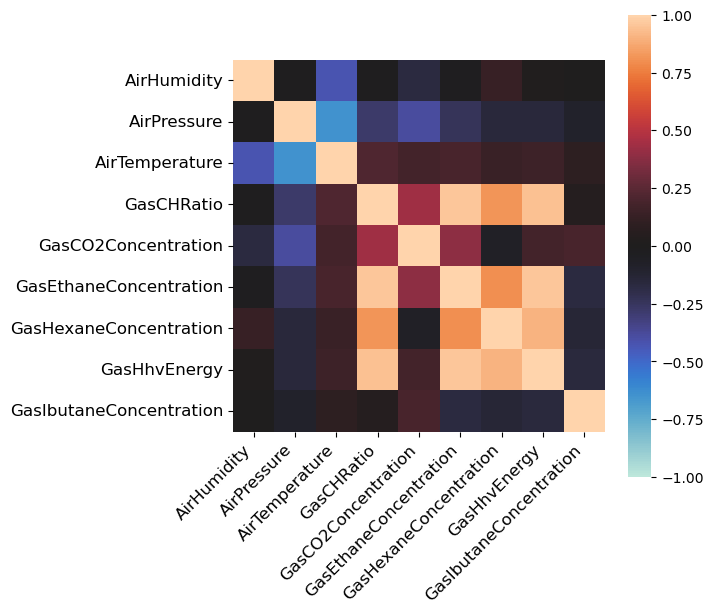
\includegraphics[scale = 0.6]{correlated_variables.png}
\end{center}


\begin{lstlisting}
corr = df.corr()
fig, ax = plt.subplots(figsize=(6,6))         
ax = sns.heatmap(corr, vmin=-1, vmax=1, center=0, square=True)
ax.set_xticklabels(
    ax.get_xticklabels(),
    rotation=45,
    horizontalalignment='right'
);
plt.show()
\end{lstlisting}






* Variables that are highly correlated (above 0.4) can be removed to avoid multicolinearity.
In the precedent correlation matrix the variables GasCHRatio, GasEthaneConcentration, GasHexaneConcentration,
GasHhvEnergy are highly correlated. We can choose to keep only one of them , GasCHRatio for instance.

\begin{lstlisting}
df.drop(['GasEthaneConcentration', 'GasHexaneConcentration',
'GasHhvEnergy'], axis=1, inplace=True)
\end{lstlisting}

  Sometimes, one needs to apply PCA in order to decorrelate the variables to feed to the classifiers. This might although make us loose interpretability.
 
\begin{lstlisting}
from sklearn.decomposition import PCA
X   = X.fillna(0)
n   = len(X.columns)
pca = PCA(n_components=n)
pca.fit(X)
fig, ax = plt.subplots(figsize=(10, 3))
ax.scatter(np.arange(n), pca.explained_variance_ratio_)
ax.set_xticks(np.arange(n))
ax.set_xticklabels(np.arange(n), fontsize=18)
ax.set_yticklabels(ax.get_yticklabels(), fontsize=14);
ax.set_ylabel('% explained variance', fontsize=14);
ax.set_title('PCA', fontsize=14);
\end{lstlisting}

\begin{center}
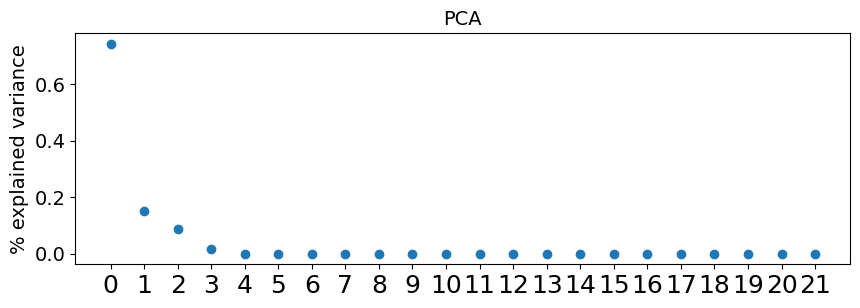
\includegraphics[scale = 0.6]{pca.png}
\end{center}




5- Partially redundant variables.


* It can be that variables are in a relationship of inclusion. For instance you may have a variable 'working day' and a variable 'holiday'. The variable 'holiday' is included in the variable 'working day' = False, but it is not equal since there are days in which you don't work and in which there are no holidays (week-ends). In this case, for predicting the traffic you might consider to keep only the variable 'working day' or to keep both variables 'working day' and 'holiday'.




4- Identify, variable by variable if it is categorical,  ordinal or numerical. 

If it is not numerical and it comes as strings, you have first to encode it, assigning a number to each observation. 

When variables are binary, but come as text convert them to numbers:
\begin{lstlisting}
from sklearn.preprocessing import LabelEncoder
le     = LabelEncoder()
label  = le.fit_transform(df['Sex'])
df["Sex_n"] = label
\end{lstlisting}


If the variables are ordinal:

\begin{lstlisting}
size_mapping = {'XXS': 1, 'XS': 2, 'S': 3, 'M': 4, 'L': 5, 'XL': 6, 'XXL': 7, 'XXXL': 8}
df['Size_Ordinal'] = df['Size'].map(size_mapping)
\end{lstlisting}




If the variables are categorical, tranform a column with n categories in n columns with indicator variables. This is also known as dummy coding and as one-hot encoding. 

\begin{lstlisting}
df_onehot = pd.get_dummies(df[["color"]], columns=['color'], dtype='int64')  
df_concat = pd.concat([df, df_onehot], axis=1)
df = df_concat.drop(columns=['color'])
\end{lstlisting}

If in a variable there is order, but this order is not monotonous, as in the case of the seasons (winter, spring, summer, and autumn), transform the observations into indicator variables. 

\section{Data overview}

To be convinced about the pertinence of using a certain variable to predict an outcome, we can plot it against the outcome, and see if we see some predictive power in the variable by itself.

There are three kinds of variables- numerical, ordinal and categorical- and two kinds of tasks -regression and categorization, and therefore two types of predicted variables discrete and continuous. In theory, there are then six ways to plot the data for a single variable analysis. Nonetheless, due to the redundancies, there are only three: 

\subsection{Numerical data vs numerical data}
\begin{center}
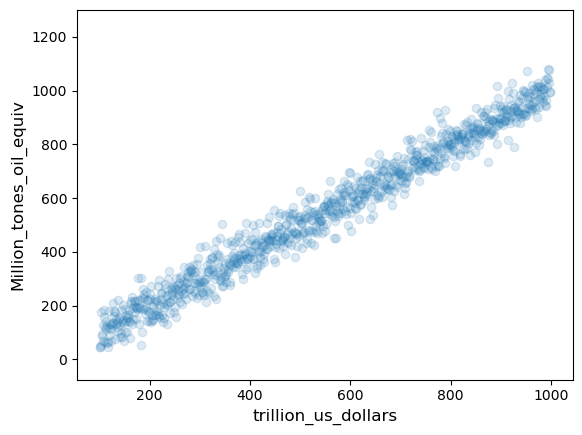
\includegraphics[scale = 0.5]{numeric_vs_numeric.png}
\end{center}

\begin{lstlisting}
fig, ax = plt.subplots()
ax.plot(df['Million_tones_oil_equiv'].values, df['trillion_us_dollars'].values,'o', alpha = 0.15 )
ax.set_xlabel('trillion_us_dollars', fontsize=12)
ax.set_ylabel('Million_tones_oil_equiv', fontsize=12)
\end{lstlisting}



We use traditional scatter plots.


\subsection{Numerical data vs discrete data}
\begin{center}
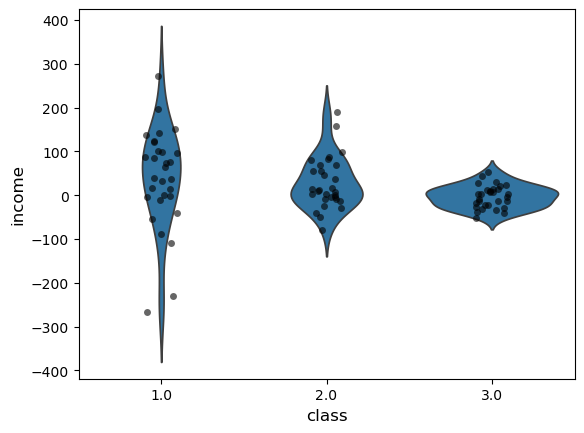
\includegraphics[scale = 0.6]{numeric_vs_discrete.png}
\end{center}

We rather use violin plots.
\begin{lstlisting}
sns.violinplot(x='class', y='income', data=df, inner=None)
sns.stripplot(x='class', y='income', data=df, color='k', alpha=0.6)
plt.xlabel('class')
plt.ylabel('income')
plt.show();
\end{lstlisting}





\subsection{Discrete data vs discrete data}
\begin{center}
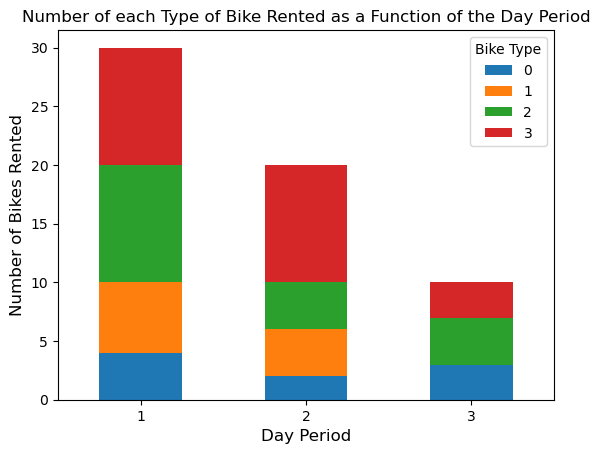
\includegraphics[scale = 0.5]{discrete_vs_discrete_0.png}
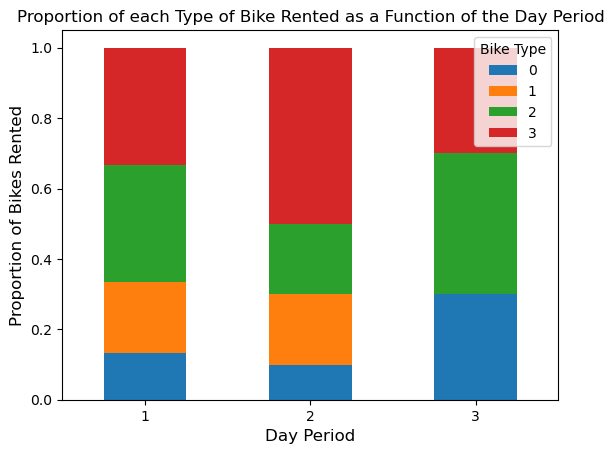
\includegraphics[scale = 0.5]{discrete_vs_discrete.png}
\end{center}
This is the more difficult one to plot. The variable was a bike of a certain category (0 to 3) and the quantity we want to predict is the day period. I choose on the left to plot the total number of bikes of each type and at right to plot the proportion of bikes rented of each type.

\begin{lstlisting}
summary = df.groupby(['day period (y)', 'bike type (x)']).size().unstack(fill_value=0)
proportions = summary.div(summary.sum(axis=1), axis=0)
summary.plot(kind='bar', stacked=True, figsize= (5,3))
plt.xlabel('Day Period')
plt.ylabel('Number of Bikes Rented')
plt.xticks(rotation=0)
plt.title('Number of each Type of Bike Rented as a Function of the Day Period')
plt.legend(title='Bike Type')
plt.show()
\end{lstlisting}



Finally, if there are not too many variables, we can have a quick global overview of several varibles at once:

\begin{lstlisting}
plt.figure(figsize=(5, 5))
axes = pd.plotting.scatter_matrix(X, alpha=0.2)
for ax in axes.flatten():
    ax.xaxis.label.set_rotation(45)
    ax.yaxis.label.set_rotation(0)
    ax.yaxis.label.set_ha('right')

plt.tight_layout()
plt.gcf().subplots_adjust(wspace=.15, hspace=.15)
plt.show()
\end{lstlisting}

\begin{center}
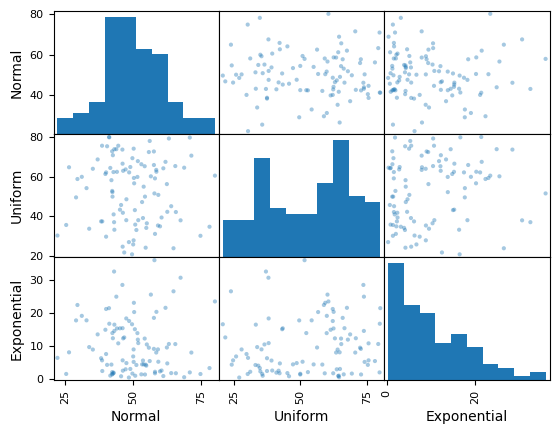
\includegraphics[scale = 0.5]{scatter_matrix.png}
\end{center}

\begin{center}
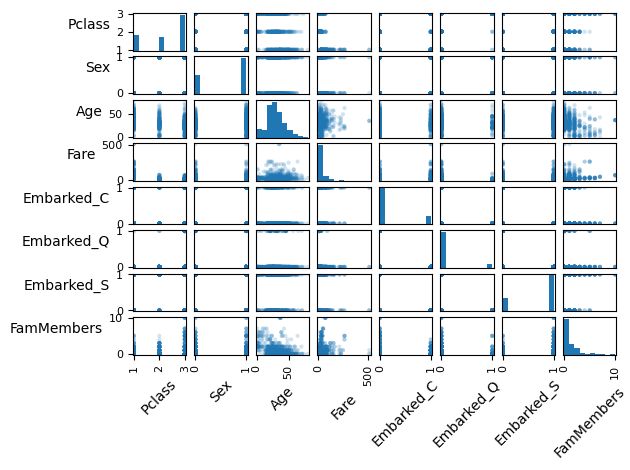
\includegraphics[scale = 0.5]{scatter_matrix_2.png}
\end{center}

\section{Data cleaning}
Cleaning consists of removing missing values, duplicates and outliers. 

\begin{lstlisting}
print(f" length of data set {len(X)}")
df.dropna(inplace=True)
print(f" length of data set {len(df)}")
df.drop_duplicates(inplace=True)
print(f" length of data set {len(df)}")
df = df[(df['column_name'] >= lower_bound) & (df['column_name'] <= upper_bound)]  
print(f" length of data set {len(df)}")
\end{lstlisting}

\subsection{Missing values}
Data cleaning might be more difficult than one thinks, in particular handling of missing values.   If the dataset is big enough (> 10000 observations) and the proportion of points with missing values is small enough with respect to the dataset size, just remove the points in which there are missing values:

\begin{lstlisting}
print(f" length of data set {len(X)}")
df.dropna(inplace=True)
print(f" length of data set {len(df)}")
\end{lstlisting}

Otherwise, removing values  has consequences as reducing the sample size, and introduce bias. An example of bias introduction is that a sensor don't send a measure when the intensity of a signal is too high. Replacing the missing value by the mean might introduce a strong bias. One could just replace the missing values by a very high value.

\begin{lstlisting}
df['sensor'].fillna(df['sensor'].mean())
\end{lstlisting}



One example of data imputation using k-nearest neighbors for a variable called 'A' in which there are missing values.

\begin{lstlisting}
from sklearn.impute import KNNImputer

imputer = KNNImputer(n_neighbors=5, weights='uniform', metric='nan_euclidean')
imputer.fit(df)
df       = pd.DataFrame(data = imputer.transform(df), columns=df.columns)
\end{lstlisting}


For categorical data, one usual strategy is to take the most frequent category. 
\begin{lstlisting}
from sklearn.impute import SimpleImputer
imputer = SimpleImputer(strategy='most_frequent')
df['A'] = pd.DataFrame(imputer.fit_transform(df[['A']]))
\end{lstlisting}


\subsection{Repeated  values}
\begin{lstlisting}
df.drop_duplicates(inplace=True)
\end{lstlisting}


\subsection{Removing outliers}

As we plotted initially single variables with respect to y, we can initially fix the range of the values that we want to observe and accept in the dataset.

\begin{lstlisting}
df = df[(df['column_name'] >= lower_bound) & (df['column_name'] <= upper_bound)]  
print(f" length of data set {len(df)}")
\end{lstlisting}

%\section{Normalizing variables}
For some algorithms, such as linear regression, logistic regression or deep networks, data normalization is used to speed up the convergence of the gradient descent, so that the cost function is isotropic, and then equally sensitive in all directions to a gradient step. In other algorithms such as decision trees, there is no need to normalize. Nonetheless, we normalize the data to be able to compare different algorithms in a same dataset.

\begin{lstlisting}
def plot_hists(df, l, c, cols, bins = 1000, figsize=(8, 5)):
    """
    Plots m histograms arranged in l lines and c columns.
    """
    m = len(cols)
    cols = list(df.columns)
    fig, axs = plt.subplots(l, c, figsize=figsize)

    for i in range(l):
        for j in range(c):
            idx = i * c + j
            if idx < m:
                axs[i, j].hist(df[cols[idx]], bins = bins)
                axs[i, j].set_title(cols[idx])          
            else:
                axs[i, j].axis("off")
    
    fig.tight_layout()
    plt.show()
\end{lstlisting}

\begin{center}
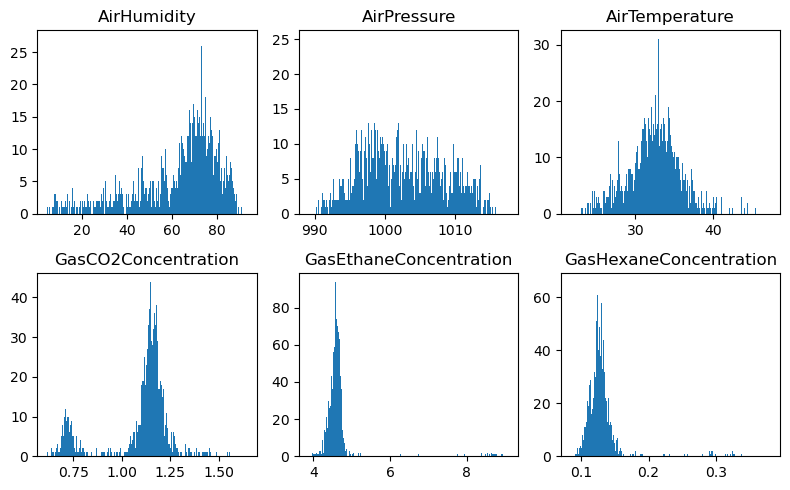
\includegraphics[scale = 0.6]{histograms_input.png}
\end{center}
First of all, we only normalize numerical values, we don't normalize ordinal nor indicator variables. Then, it depends a bit on the distribution of each variable.

When the data looks already Gaussian, just z-score using StandardScaler. For skewed distributions use rather PowerTransformer (in it's two flavours  Box-Cox and Yeo-Johnson). QuantileTransformer,  is able to cope with several outliers, but is not suited for small datasets. MinMaxScaler is rather used to normalize between 0 and 1. This last scaler is often used for images, of in cases in which the data themselves are bounded, and look approximately uniform.

It is very important to observe the histograms before and after normalization, since the method employed can disrupt fundamental features of the original distribution. For instance, when applying a quantile distribution on a bimodal distribution, we end with a unimodal distribution. 
 As a rule of thumb, the first normalizer you should have in mind is the PowerTransformer, it will transform a Gaussian into a Gaussian, an uniform into an uniform, a lognormal into a normal.





\begin{lstlisting}
from sklearn.preprocessing import PowerTransformer
df_norm = df.copy()
scaler = PowerTransformer()
for var in list(df_norm.columns):
    df_norm[[var]] = scaler.fit_transform(df_norm[[var]].values.reshape(-1, 1))
\end{lstlisting}


\begin{center}
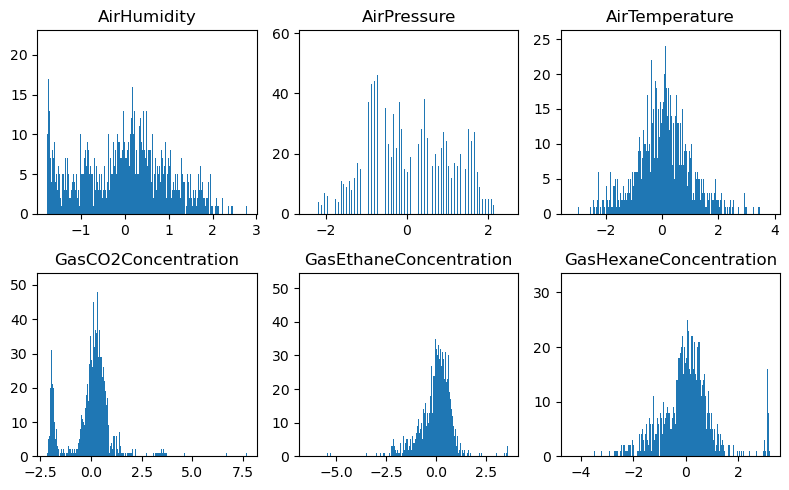
\includegraphics[scale = 0.6]{histograms_output.png}
\end{center}

%\section{Dataset balance}
In classification tasks it is crucial for certain tasks like crossvalidation and assessing baseline performance, to determine whether a dataset is balanced or imbalanced. A dataset is balanced when each category has the same number of elements n, and it's imbalanced when one category is overrepresented or underrepresented with respect to n.
A quick way to visualize this is by doing a barplot.

\begin{lstlisting}
labels, counts = np.unique(y, return_counts=True)
plt.figure(figsize=(8,3)) 
plt.bar(labels, counts, align='center', facecolor = '#2ab0ff', width=0.4)
\end{lstlisting}




\section{Baseline models}
  
  Dummy or baseline models are a way to establish a baseline to how well a classification model is performing. For instance if there are 90 percent of binary labels y that are equal to 1 (and 10 percent equal to 0). A model that, disregarding all the input features,  always outputs 1 will have a 90 percent performance. Therefore a model that has a performance that is lower than 90 percent will be a terrible model.
    
\begin{lstlisting}
from sklearn.dummy import DummyClassifier
from sklearn.metrics import recall_score, precision_score, f1_score
dummy_clf = DummyClassifier(strategy="most_frequent")
dummy_clf.fit(X, y)
y_pred = dummy_clf.predict(X)
print(f'Recall: {recall_score(y, y_pred)}')
print(f'Precision: {precision_score(y, y_pred)}')
print(f'F1-score: {f1_score(y, y_pred)}')
\end{lstlisting}  

\section{Crossvalidation}

Crossvalidation is a statistical method used to estimating model performance and tuning hyperparameters. 
By dividing the dataset over and over into several non overlaping segments, we train the model in fixed proportions like 60/40 or 80/20 percent. The model is trained on the first part and evaluated on the second in such a way that we evaluate the model on data in which the model hasn't been trained. This is called  evaluating it's generalization performance. 
By generalisation performance, we should think about a polynom that you fit using 5 points $x_1, x_2, ..., x_5, x_1 < x_2 ... < x_5$ and then you want to know how well the model interpolates  in points in which is hasn't been trained (but of course you evaluate points in the interval $]x_1, x_5[$), you are not interested in extrapolating, ie in points higher than $x_5$ or lower than $x_1$. The degree to which your model will approximate the underlying manifold over which there is noise, depends on the level of noise, and on the match between our model complexity and the manifold complexity.

%For very imbalanced datasets, like the one described in the paragraph baseline models, the models performance is not going to show it's potential when trained: it's going to be biased and be inaccurate. 


\begin{lstlisting}  
from sklearn.model_selection import StratifiedKFold
skf = StratifiedKFold(n_splits=5, shuffle=True, random_state=42)
for train_index, test_index in skf.split(X, y):
    X_train, X_val = X[train_index], X[test_index]
    y_train, y_val = y[train_index], y[test_index]
# train on training set, eval on validation set 
\end{lstlisting}  

One can also oversample the minority class to match the majority class (here using the Imbalanced-learn library). You can also check out also 'smote' in imblearn.

\begin{lstlisting}  
from imblearn.over_sampling import RandomOverSampler
from collections import Counter
ros = RandomOverSampler(random_state=42)
X_resampled, y_resampled = ros.fit_resample(X, y)
print("Oversampled class distribution:", Counter(y_resampled))
\end{lstlisting}  


The most currently used one, for tabular data in which the observations are independent the ones from the other, and in the case in which the dataset is balanced is known as shuffle split cross-validation or Monte Carlo crossvalidation, in which the partitions are selected at random. Another close technique (in which there is no randomness involved) is K-fold crossvalidation, in which the data is split K times, and use one of the folds as test set and the rest as training set: in total the model is trained and evaluated k times.

\begin{lstlisting}  
from sklearn.model_selection import GridSearchCV, StratifiedKFold

param_grid_rf = {'n_estimators': [100, 200], 'max_depth': [None, 5, 10]}
param_grid_svm = {'C': [0.1, 1, 10], 'kernel': ['linear', 'rbf']}
outer_cv = StratifiedKFold(n_splits=5, shuffle=True, random_state=15)
inner_cv = StratifiedKFold(n_splits=3, shuffle=True, random_state=1)
rf_model = RandomForestClassifier()
svm_model = SVC()
rf_scores = []
svm_scores = []
for train_outer, test_outer in outer_cv.split(X, y):
  X_outer_train, X_outer_test = X[train_outer], X[test_outer]
  y_outer_train, y_outer_test = y[train_outer], y[test_outer]
  for train_inner, test_inner in inner_cv.split(X_outer_train, y_outer_train):
    X_inner_train, X_inner_test = X_outer_train[train_inner], X_outer_train[test_inner]
    y_inner_train, y_inner_test = y_outer_train[train_inner], y_outer_train[test_inner]
    rf_grid = GridSearchCV(rf_model, param_grid_rf, cv=inner_cv)
    svm_grid = GridSearchCV(svm_model, param_grid_svm, cv=inner_cv)
    rf_grid.fit(X_inner_train, y_inner_train)
    svm_grid.fit(X_inner_train, y_inner_train)
    rf_best_model = rf_grid.best_estimator_
    svm_best_model = svm_grid.best_estimator_
    rf_score = rf_best_model.score(X_outer_test, y_outer_test)
    svm_score = svm_best_model.score(X_outer_test, y_outer_test)
    rf_scores.append(rf_score)
    svm_scores.append(svm_score)

print("Average Random Forest score:", np.mean(rf_scores), "Average SVM score:", np.mean(svm_scores))

best_model = rf_grid.best_estimator_
X_train, X_test, y_train, y_test = train_test_split(X, y, test_size=0.2, random_state=42)
best_model.fit(X_train, y_train)
y_pred = best_model.predict(X_test)  
\end{lstlisting}  


Over the learning process, weights get adjusted and a cost function is minimized. The testing error therefore reflects the generalization performance. Nonetheless, if we only train once and evaluate afterwards which hyperparameter performs better on the test data, we might be over-fitting the model on this dataset. This is why in the previous code, we did a nested crossvalidation: in the inside loop (GridSearchCV) one minimizes the cost function in different partitions of the data for different hyperparameters, and retain the estimator / model which performs better. It is a good practice to use present balanced data to the models in this internal loop, this is why we did stratified crossvalidation. Then, in the outer loop, we evaluate the model on the test data.

In the following, I present a faster version of the crossvalidation (without nested crossvalidation).

\begin{lstlisting}  
models = {"Random Forest": RandomForestClassifier(),
    "Gradient Boosting": GradientBoostingClassifier(),}
param_grids = {
    "Random Forest": {'n_estimators': [100, 200, 300], 'max_depth': [None, 5, 10]},
    "Gradient Boosting": {'n_estimators': [100, 200, 300], 'learning_rate': [0.1, 0.05, 0.01]},}
best_model = None
best_score = 0
for model_name, model in models.items():
    grid_search = GridSearchCV(model, param_grids[model_name], cv=5)
    grid_search.fit(X_train, y_train)
    score = grid_search.best_score_
    print(f"{model_name}: Best score = {score:.3f}")
    if score > best_score:
        best_model = grid_search.best_estimator_
        best_score = score
best_model.fit(X_train, y_train)
y_pred = best_model.predict(X_test)   

accuracy = accuracy_score(y_test, y_pred)
precision = precision_score(y_test, y_pred)
recall = recall_score(y_test,   
 y_pred)
f1 = f1_score(y_test, y_pred)
print(f"Best   
 Model: {type(best_model).__name__}")
print(f"Accuracy: {accuracy:.3f}")
print(f"Precision: {precision:.3f}")
print(f"Recall: {recall:.3f}")
print(f"F1-score: {f1:.3f}"
\end{lstlisting}  


\section{Combining models to improve accuracy}
 
In here we present voting, the simplest way of combining models. There exists another technique called ensemble learning (Bagging, Boosting, Stacking).

\begin{lstlisting}  
from sklearn.ensemble import RandomForestClassifier, AdaBoostClassifier, VotingClassifier
from sklearn.model_selection import cross_val_score   
rf = RandomForestClassifier(n_estimators=100)
ada = AdaBoostClassifier(n_estimators=100)
voting_clf = VotingClassifier(estimators=[('rf', rf), ('ada', ada)], voting='hard')
scores = cross_val_score(voting_clf, X_train, y_train, cv=5)
print("Accuracy:", scores.mean())
\end{lstlisting}  



\section{Data leakage}

Data leakage usually happens when we don't split appropriately the data set in training, validation and test set, so that we don't evaluate the model's performance on data that was used to train.
The second more frequent source of data leakage often happens in more subtle ways, usually when we use variables which contain information about the variable being predicted, in undesired ways: if the variables that you use didn't contained information/ hints about the predicted variables, you wouldn't want to consider this variable. But the problem precisely comes when the variables contain too much information. We 
 expect from a classifier that it combines non-linearly features which by themselves have low predictive power. For instance, for medical diagnosis, we would like to say how likely one person can have a certain decease. Taken by one by one, variables like age, income, smoking, occupation,  dietary habits, sport practice ... have low predictive power on a decease like lung cancer, and it's the combination of these features which helps to make an accurate prediction.
 

Also, we want the prediction process to be "feedforward", and not having predicting variables that are function of the output. Coming back to our example of decease prediction, if you include a feature like name of previous treatments, this might already be a high about patient condition. When creating new variables/ features (this is called feature engineering), one combines existing variables in non-linear ways. Nonetheless, it can happen that when creating a feature like $a.(x_1-m)^2 + bx_2 + c$, in which $x_1$ and $x_2$ are variables, one introduces parameters like $m$ which might have information about the variable being predicted. 

When dealing with time series there are systematic risks of data leakage, since there are temporal dependencies in the data: the value at a given point depends, for continuity reasons of the values of precedent data points. For time series, crossvalidation is done in a particular way called time series crossvalidation, in which the data split into consecutive time periods, so that the prediction makes sense (since the mean and the variance of a signal may change over time), and that we avoid data leaking.


Some red flags for identify data leakage are having a model performance that is too high, or variable weights that are also too important. During crossvalidation, you can print the performance on the training and on the testing set. If the model performs significantly better on the testing set, it might well be due to data leakage. 
 
\begin{lstlisting}  
grid_search = GridSearchCV(model, param_grid, cv=5)   
grid_search.fit(X_train, y_train)
train_predictions = grid_search.best_estimator_.predict(X_train)
train_accuracy = accuracy_score(y_train, train_predictions)
test_predictions = best_model.predict(X_test)
test_accuracy = accuracy_score(y_test, test_predictions) 
\end{lstlisting}  

 

\section{Grid search on models}

In the following, I provide some starting parameters for the grid hyperparameter search of different models. When the number of hyperparameters is too large use rather RandomizedSearchCV.

\subsection{Classification Models}
\subsubsection{Logistic regression}


\begin{lstlisting}
param_grid = {'penalty': ['elasticnet'], 'C':[0.001, 0.01, 0.1, 1, 10],             
              'class_weight': ['balanced',None], 'l1_ratio':  [0.1, 0.3, 0.5, 0.7, 0.9, 1], 'max_iter': [5, 7, 10, 20], 'solver':['saga']}
lr_estimator = LogisticRegression()
\end{lstlisting}

This grid search is only a a starting point: if for instance you obtain the best performance  for the regularisation parameter 'C' is 10, rerun a grid search with  'C':[5, 10, 50, 100, 1000], since C= 10 is at the border of the proposed interval.

\subsubsection{Random forest classification}

\begin{lstlisting}
param_grid_rf = {
    'n_estimators': [100, 200, 300], 
    'max_depth': [None, 5, 10], 
    'min_samples_split': [2, 5, 10],
    'min_samples_leaf':  [1, 2, 4],
    'max_features': ['auto', 'sqrt', 'log2'],  
    'bootstrap': [True, False]
}
\end{lstlisting}


\subsubsection{Support vector machine (SVM)}

\begin{lstlisting}
param_grid_svm = {
    'C': [0.001, 0.01, 0.1, 1, 10],
    'kernel': ['linear', 'poly', 'rbf', 'sigmoid'],
    'degree': [2, 3, 4], 
    'gamma': ['scale', 'auto']
}
\end{lstlisting}

\subsubsection{Gradient Boosting machine (GBM)}

\begin{lstlisting}
param_grid_gbm = {
    'n_estimators': [100, 200, 300],
    'learning_rate': [0.1, 0.05, 0.01],
    'max_depth': [3, 5, 7],
    'subsample': [0.8, 0.9, 1.0],
    'min_samples_split': [2, 5, 10],
    'min_samples_leaf': [1, 2, 4]
}
\end{lstlisting}

\subsubsection{XGB Classifier}
from xgboost import XGBClassifier
\begin{lstlisting}
param_grid_xgb = {
    'n_estimators': [200, 500, 600],
    'learning_rate': [0.01, 0.07, 0.1, 0.3],
    'max_depth': [7, 13, 15],
    'grow_policy': ['depthwise', 'levelwise'],
    'colsample_bytree': [0.5, 0.7, 1.0],
    'colsample_bylevel': [0.5, 0.7, 1.0],
    'colsample_bynode': [0.5, 0.7, 1.0],
    'importance_type': ['weight', 'gain', 'cover'],
}
\end{lstlisting}


\subsection{Regression models}


\subsubsection{Lasso (L1)}
\begin{lstlisting}
param_grid_lasso = {
    'alpha': [0.001, 0.01, 0.1, 1, 10],
    'fit_intercept': [True, False],
    'normalize': [True, False]
}
\end{lstlisting}

\subsubsection{Random forest regressor}

\begin{lstlisting}
     param_grid_rf_reg = {
    'n_estimators': [100, 200, 300],
    'max_depth': [None, 5, 10],
    'min_samples_split': [2, 5, 10],
    'min_samples_leaf': [1, 2, 4],
    'max_features': ['auto', 'sqrt', 'log2'],
    'bootstrap': [True, False]}
\end{lstlisting}



\subsection{Evaluation metrics}

\subsubsection{Classification metrics}


\begin{lstlisting}
from sklearn.metrics import accuracy_score, precision_score, recall_score, f1_score, confusion_matrix, classification_report, roc_curve, auc   
accuracy = accuracy_score(y_true, y_pred)
precision = precision_score(y_true, y_pred)
recall = recall_score(y_true, y_pred)
f1 = f1_score(y_true, y_pred)   
conf_matrix = confusion_matrix(y_true, y_pred)   
report = classification_report(y_true, y_pred)
fpr, tpr, thresholds = roc_curve(y_true, y_pred)
roc_auc = auc(fpr, tpr)
print(f"Accuracy: {accuracy}, Precision: {precision}, Recall: {recall}, F1-score: {f1}" )
print("Confusion matrix:\n", conf_matrix)
print("Classification report:\n",   
 report)
print("AUC:", roc_auc)
\end{lstlisting}


\subsubsection{Regression metrics}
There are several metrics that quantify the difference in area between the target variable and the regression model.

\begin{lstlisting}
from sklearn.metrics import mean_squared_error, mean_absolute_error, r2_score
mse = mean_squared_error(y_true, y_pred)
rmse = mean_squared_error(y_true, y_pred, squared=False)
mae = mean_absolute_error(y_true, y_pred)
r2 = r2_score(y_true, y_pred)
\end{lstlisting}


\subsection{Feature importance}
One often wants to assess what is the importance of each feature on the final outcome. 


For linear regression:
\begin{lstlisting}
labels = model_LR.feature_names_in_
fig, ax = plt.subplots(figsize=(10, 3))
ax.plot(model_LR.coef_,'.')
plt.xticks(np.arange(len(model_LR.coef_)), labels, rotation = 45);
\end{lstlisting}


For random forests:
\begin{lstlisting}
grid_search = GridSearchCV(estimator=model_RF, param_grid=parameters, cv=5)
grid_search.fit(X_train, y_train)
importances = grid_search.best_estimator_.feature_importances_
std = np.std([tree.feature_importances_ for tree in grid_search.best_estimator_.estimators_], axis=0)
forest_importances = pd.Series(importances, index=grid_search.best_estimator_.feature_names_in_)
fig, ax = plt.subplots()
forest_importances.plot.bar(yerr=std, ax=ax)
ax.set_title("Feature importances")
ax.set_ylabel("Mean decrease in impurity")
fig.tight_layout()
\end{lstlisting}


\section{AutoML}

\begin{lstlisting}
import autosklearn.classification
automl = autosklearn.classification.AutoSklearnClassifier()
    automl.fit(X_train, y_train)
    y_hat = automl.predict(X_test)
\end{lstlisting}


\section{Industrialization}

\subsection{Methodology}
Industrializing a machine learning model is a big subject.
Besides from the usual guidelines for project development (clean code, version control, unitary tests), machine learning projects have some specificities.
 In addition to the previously covered that includes the data preparation  and the model development, there are additional steps: 
 
- Model deployment: choose an adequate architecture (internal server, cloud server) and deploy the model, for instance using an API rest in containers (Docker) and in container orchestrators (Kubernetes). 
These containers can be deployed locally or in the cloud.  

- Monitor model's performance: if there is data drift, the model's performance will drop. Therefore, the model will have to be retrained.  Check existing monitoring tools like MLflow and Kubeflow.

\subsection{Create a simple API rest for a machine learning model}

In order to use a model in a production environment, one has to feed it with data and retrieve the predictions in order to be used. REST API's allow different software applications to interact using http requests.

An endpoint is an URL to which a user can send requests and receive back responses thought different methods (get, post, put, ...).

\subsubsection{Development phase: off-line model creation}

\begin{lstlisting}
from sklearn.linear_model import LinearRegression
from sklearn.preprocessing import PowerTransformer
import pandas as pd
import joblib
import json
import requests

norm_A = PowerTransformer(method='yeo-johnson', standardize=True)
X_norm[['A']] = norm_A.fit_transform(X_norm[['A']].values.reshape(-1, 1))
norm_B = PowerTransformer(method='yeo-johnson', standardize=True)
X_norm[['B']] = norm_B.fit_transform(X_norm[['B']].values.reshape(-1, 1))

model = LinearRegression()
model.fit(X_norm, y)

joblib.dump(norm_A, 'norm_A.pkl');
joblib.dump(norm_B, 'norm_B.pkl');
joblib.dump(model, 'model.pkl')
\end{lstlisting}



\subsubsection{app.py: creation of a endpoint called '/predict'}

\begin{lstlisting}
from flask import Flask
from flask_restful import Api, Resource, reqparse
import joblib
import numpy as np
import json
import pandas as pd
APP = Flask(__name__)
API = Api(APP)

model    = joblib.load('model.pkl')
norm_A   = joblib.load('norm_A.pkl')
norm_B   = joblib.load('norm_B.pkl')
class Predict(Resource):
    @staticmethod
    def post():
        parser = reqparse.RequestParser()
        parser.add_argument("A", type=float, required=True)
        parser.add_argument("B", type=float, required=True)
        args = parser.parse_args()
        args_norm = args.copy()
        args_norm["A"] = norm_A.transform(np.array([[args["A"]]]))[0][0]
        args_norm["B"] = norm_B.transform(np.array([[args["B"]]]))[0][0]
        pred = model.predict(pd.DataFrame(data = args_norm, index = [0]))[0]
        out = json.dumps({'Prediction': pred.tolist()})
        return out, 200

API.add_resource(Predict, '/predict')
if __name__ == '__main__':
    APP.run(debug=True, port='1080')
\end{lstlisting}

\subsubsection{Server launch}
Create a conda environment, include flask, joblib, json, numpy, pandas, sklearn, flask restful, requests. In this environment, run in the bash the script app.py.
\begin{lstlisting}
python app.py
\end{lstlisting}


\subsubsection{Request creation}


\begin{lstlisting}
request = {
           "A": 0.47,
           "B": -0.352,
           }

data_json = json.dumps(request)
response  = requests.post('http://127.0.0.1:1080/predict', data=data_json, headers= {'Content-Type': 'application/json'})
json_data = json.loads(response.json())
prediction = json_data["Prediction"][0]
\end{lstlisting}


\section{Appendix: useful commands}

\subsection{Usual imports}
\begin{lstlisting}
from sklearn.preprocessing import LabelEncoder
from sklearn.impute import SimpleImputer, KNNImputer
from pandas.plotting import scatter_matrix
from sklearn.preprocessing import PowerTransformer
from sklearn.dummy import DummyClassifier
from sklearn.metrics import recall_score, precision_score, f1_score, accuracy_score

from sklearn.ensemble import GradientBoostingClassifier, RandomForestClassifier
from sklearn.model_selection import GridSearchCV
\end{lstlisting}



\subsection{File loading}
\begin{lstlisting}
df = pd.read_csv('../data/train.csv')
\end{lstlisting}


\subsection{Data frame concatenation}
\begin{lstlisting}
df_c = pd.concat([df1, df2], axis=1)
\end{lstlisting}



\subsection{Exporting dataframe to csv}
\begin{lstlisting}
df.to_csv('Kaggle_1.csv', index = False)
\end{lstlisting}



\bibliographystyle{unsrtnat}
\bibliography{references}


\end{document}







